\documentclass[12pt,a4paper,conference]{IEEEtran}
\usepackage[utf8]{inputenc}
\usepackage[english]{babel}
\usepackage{amsmath}
\usepackage{amsfonts}
\usepackage{amssymb}
\usepackage{graphicx}
\usepackage{subcaption}

\usepackage{float}
\usepackage{fullpage}

\usepackage[hidelinks]{hyperref}

\usepackage{tikz}
\usepackage{fp} %floating point package

\usepackage{todonotes}
\usepackage{epstopdf}
\usepackage{graphicx}
\usepackage[T1]{fontenc}


\let\ig\includegraphics
\renewcommand{\includegraphics}[2][]{ \IfFileExists{#2}{ \ig[#1]{#2} }{ 
		\IfFileExists{#2.eps}{ \ig[#1]{#2} }{ 
		\IfFileExists{#2.png}{ \ig[#1]{#2} }{ 
		\IfFileExists{#2.jpg}{ \ig[#1]{#2} }{ 
		\IfFileExists{#2.jpeg}{ \ig[#1]{#2} }{ 
		\IfFileExists{#2.gif}{ \ig[#1]{#2} }{ 
		\IfFileExists{#2.ppm}{ \ig[#1]{#2} }{ 
		\missingfigure{  \protect\detokenize{#2} was not found.} 
}}}}}}}
}

\newcommand{\missingequation}[1]{\todo[inline, color = yellow]{Missing equation: #1}}


%%
%% End of file `mypackage.sty'.

\newcommand{\cutOutWidth}{0.45 \linewidth}
\newcommand{\histogramWidth}{0.8 \linewidth}
\newcommand{\fullImageWidth}{0.8 \linewidth}


\begin{document}
\raggedbottom

\title{Visual Servoing\\ \large{ROVI - Finalproject}}
\author{Nikolaj Iversen and Lukas Schwartz}
\date{18$^{th}$ December 2015}

\maketitle

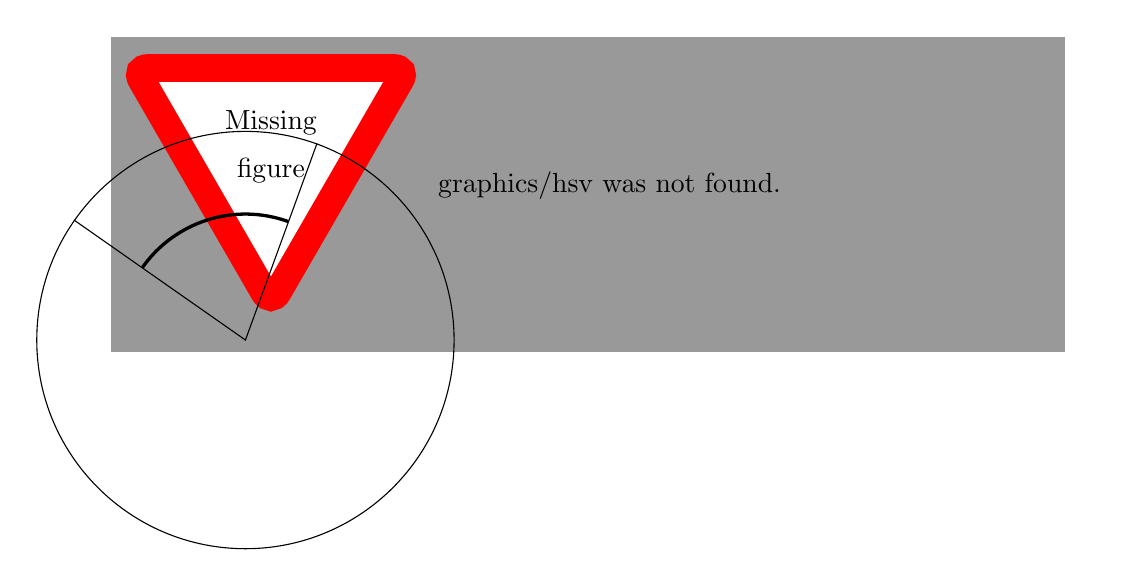
\begin{tikzpicture}
 \node {\includegraphics[scale=1]{graphics/hsv} };
 \node[name=hsv, draw, circle, minimum width =5.3cm] at (-4,-1.85) {};
% % % % RED % % % %
% \newcommand{\MinHue}{0} %angle
% \newcommand{\MaxHue}{30}
% \newcommand{\MinSat}{1.6cm} % 0 - 1 => 0 - 2.65
%  \draw (hsv.\MinHue) -- (hsv.center) -- (hsv.\MaxHue);
%  \draw[very thick]   ([shift=(\MinHue:\MinSat)] hsv.center) arc(\MinHue:\MaxHue:\MinSat);
% % % % GREEN % % % %
\newcommand{\MinHue}{70} %angle 
\newcommand{\MaxHue}{145}
\newcommand{\MinSat}{1.6cm} % 0 - 1 => 0 - 2.65
 \draw (hsv.\MinHue) -- (hsv.center) -- (hsv.\MaxHue);
 \draw[very thick]   ([shift=(\MinHue:\MinSat)] hsv.center) arc(\MinHue:\MaxHue:\MinSat);
% % % % BLUE % % % %
% \newcommand{\MinHue}{210} %angle
% \newcommand{\MaxHue}{270}
% \newcommand{\MinSat}{1.6cm} % 0 - 1 => 0 - 2.65
%  \draw (hsv.\MinHue) -- (hsv.center) -- (hsv.\MaxHue);
%  \draw[very thick]   ([shift=(\MinHue:\MinSat)] hsv.center) arc(\MinHue:\MaxHue:\MinSat);

\end{tikzpicture}


\begin{tikzpicture}
 \newcommand{\angleA}{10}
 \newcommand{\radiuA}{1}
 \newcommand{\radiuB}{1}
 
 \FPeval{\angleB}{\angleA + 90}
 
 \node[name=image] at (0,0) {};
 
 \node[scale=0.3,fill=black, minimum width=15cm, rotate={90 + \angleA}, name=lineA] at ([shift=(\angleA:\radiuA cm)] image.center) {};
 \node[name=midA] at ($(wall.180)!(image.center)!(wall.0)$) {};
 \node[above] at (lineA.0) {line a};

 \node[scale=0.3,fill=black, minimum width=15cm, rotate={90 + \angleB}, name=lineB] at ([shift=(\angleB:\radiuB cm)] image.center) {};
 \node[name=midB] at ($(wall.180)!(image.center)!(wall.0)$) {};
 \node[above] at (lineB.0) {line b};
 
 \FPeval{\rad}{\FPpi/180} %couldn't find the function
 \FPeval{\posX}{round(cos(\angleA * \rad)*\radiuA + cos(\angleB * \rad)*\radiuB,3)}
 \FPeval{\posY}{round(sin(\angleA * \rad)*\radiuA + sin(\angleB * \rad)*\radiuB,3)}
 
 \node[draw, circle]  at (\posX,\posY) {};
\end{tikzpicture}


\end{document}